\section{DATA ANALYSIS AND DATA MINING}
\label{section:analysis}
\subsection{SQL function implementation}
\label{sect:sub-title}
Produce sample SQL queries on these relations that are used for practical daily
operations and activities 

Produce sample SQL queries on these relations which are of an analytic or data 
mining nature

Suggest which data fields of the relational schema should be indexed or 
hashed, and explain your decision

\subsection{Data Mining}
\label{sect:sub-title}
	Here, with the tools we build and the data visualization tool, Flourish, we take a look what data analysis work we can potentially using our tools.

\begin{figure}[H]
    \centering
    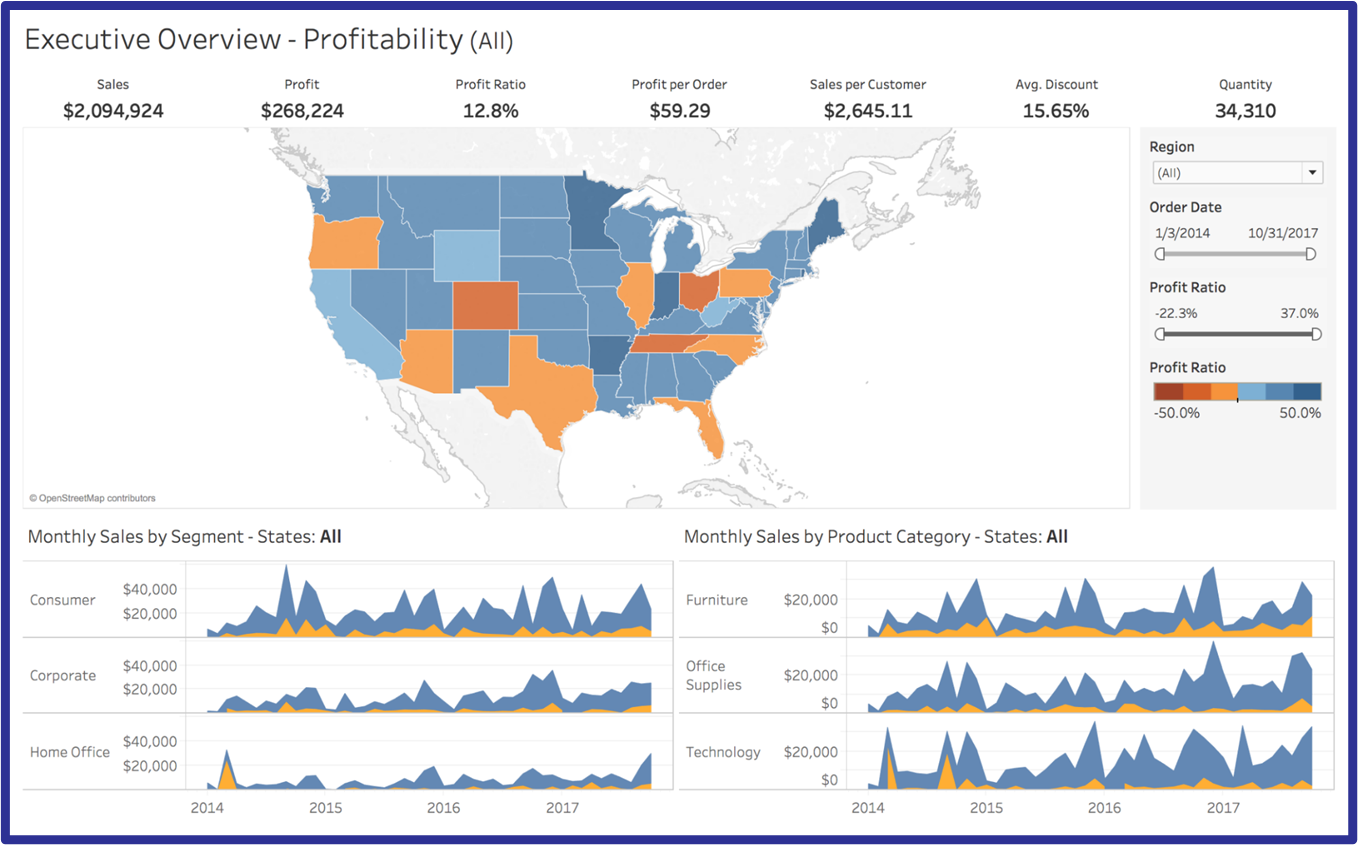
\includegraphics[width=\columnwidth]{images/DataMap.png}
    \caption[Short text]{Overview map of the data set}
    \label{fig:Overview}
\end{figure}
We can first build correlation map with our tools to give users a basic insight of the data set.

\begin{figure}[H]
    \centering
    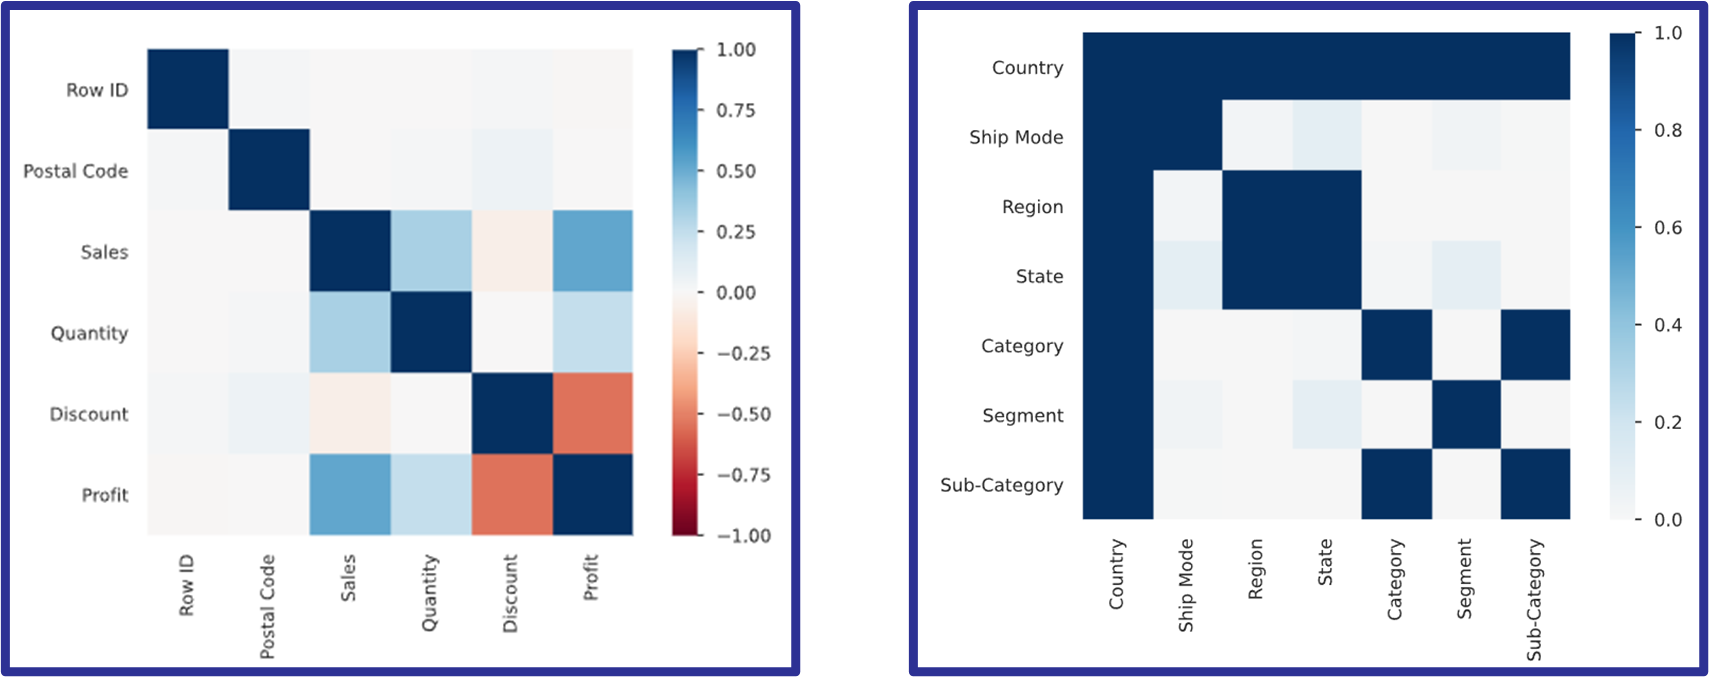
\includegraphics[width=\columnwidth]{images/correlation.png}
    \caption[Short text]{Correlation map of the data set using Spearman's and Cramér's methods}
    \label{fig:Correlation}
\end{figure}

Then, we can select an attribute that we are interested in and analyze from there. Here, we select the "category" attribute. As shown in the image below, office supplies leads in sales in the three main categories.

\begin{figure}[H]
    \centering
    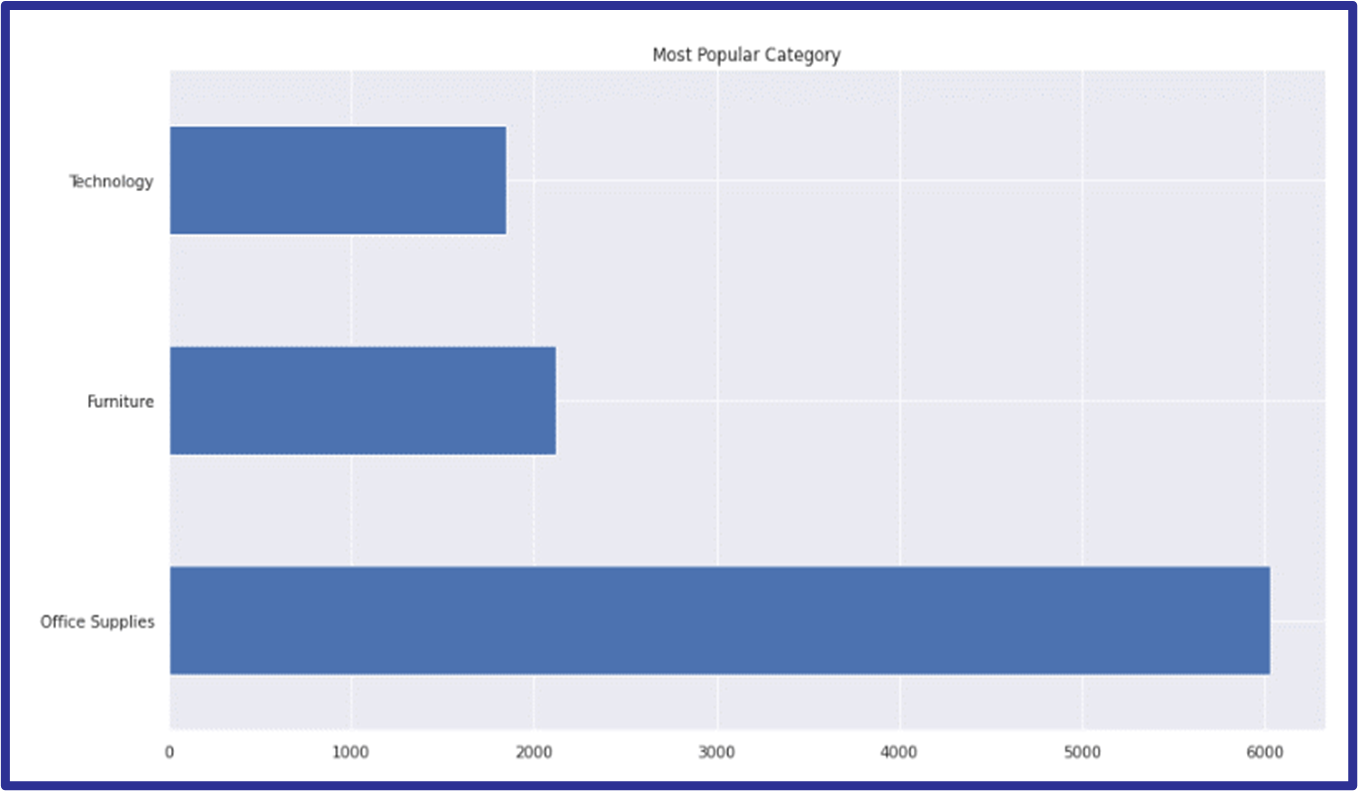
\includegraphics[width=\columnwidth]{images/cata1.png}
    \caption[Short text]{Category and Sales}
    \label{fig:Category&Sales}
\end{figure}

We can add more attributes to give users a better understanding of the data. Here, we add profit to the mix. And we can see that though office supplies has the best sales, but technology has a much better profit margin, which makes it have the highest overall profit.

\begin{figure}[H]
    \centering
    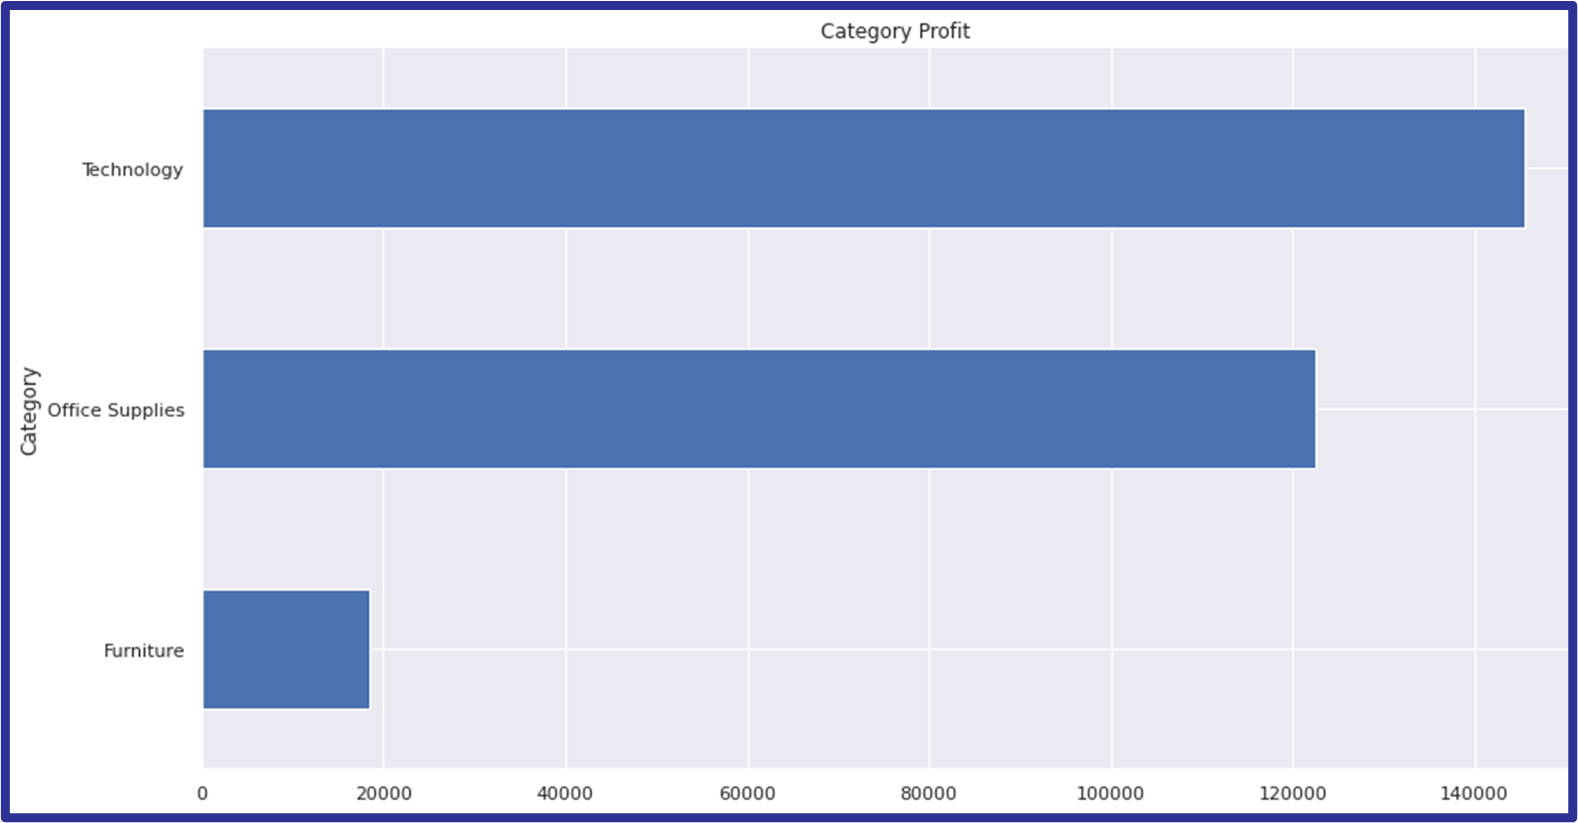
\includegraphics[width=\columnwidth]{images/cata2.png}
    \caption[Short text]{Category and Profit}
    \label{fig:Category&Profit}
\end{figure}
Also, we add the "city" attribute for a deeper analysis. We can see that New York city as the economic center of the US, it has the highest profit when it comes economic related category like "technology" and "office supplies". And Seattle, though a much smaller city than New York, has a higher profit than New York with "furniture", showing its livable suburb property as a city.
With more data like the population of each city, we can expand further and do a deeper analysis using our tools, showing great potential of our tools for data analysis and mining.

\begin{figure}[H]
    \centering
    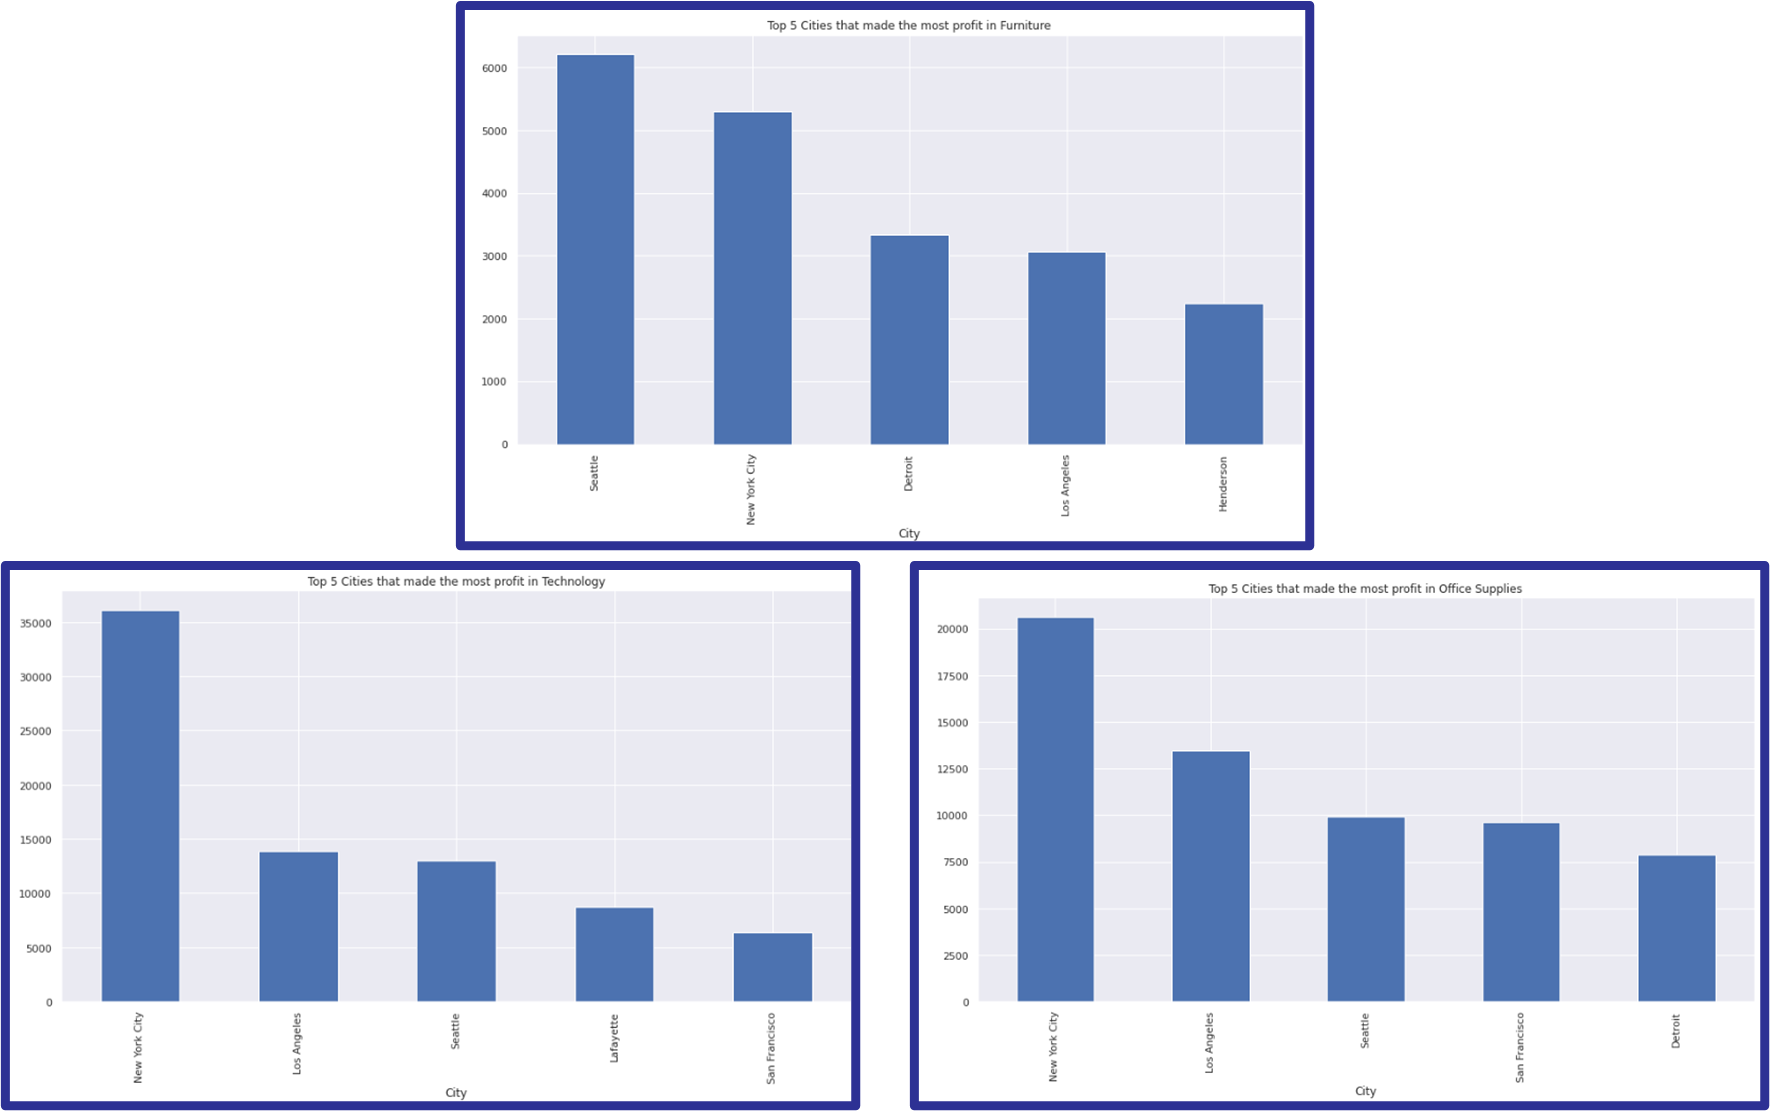
\includegraphics[width=\columnwidth]{images/cata3.png}
    \caption[Short text]{Category and Profit and City}
    \label{fig:Category&Profit&City}
\end{figure}

Additionally, we can build other useful graph, such as pie chart. Here, we build a pie chart to show the percentage of different kind of customer's contribution to sales.

\begin{figure}[H]
    \centering
    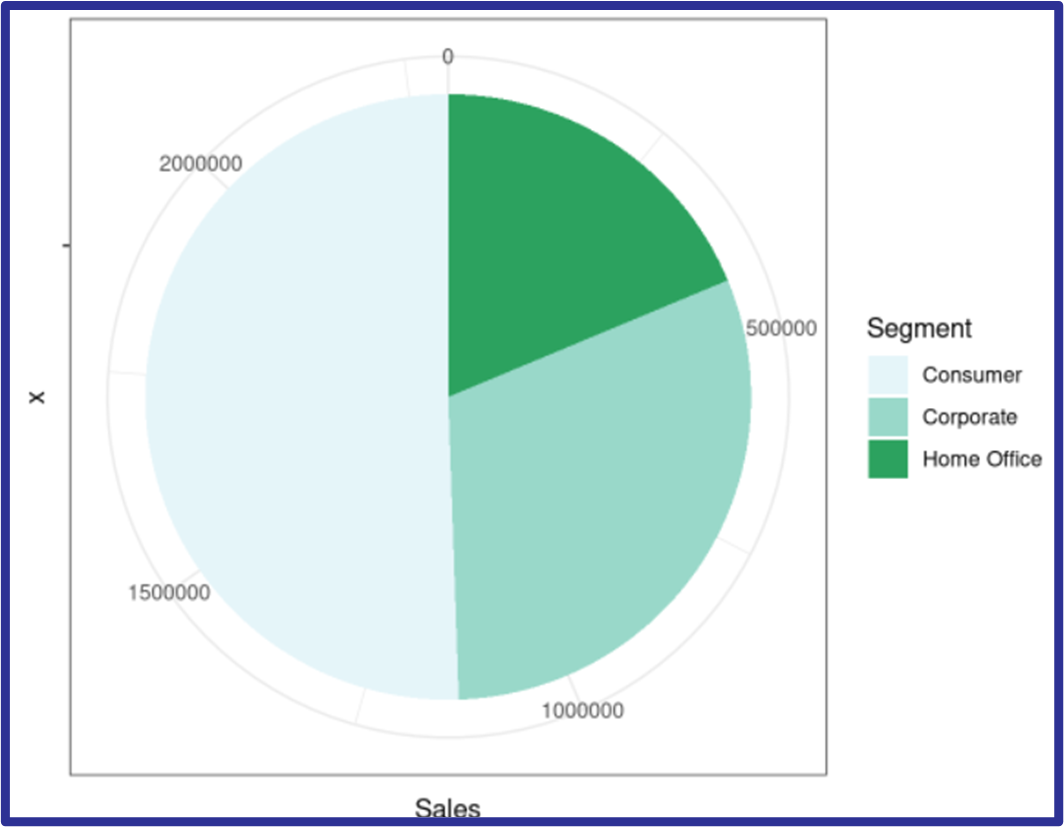
\includegraphics[width=\columnwidth]{images/pie.png}
    \caption[Short text]{Pie chart of category of customers}
    \label{fig:Pie Chart}
\end{figure}